\section{data}
\label{sec:data}

\subsection{The MaNGA survey}

MaNGA is one of the three core programs in the fourth-generation Sloan Digital Sky Survey (SDSS-IV) which began on July, 2014 \citep{2015ApJ...798....7B, drory_manga_2015}, it employs the Baryon Oscillation Spectroscopic Survey (BOSS) spectrographs \citep{smee_multi-object_2013} on the 2.5m Sloan Foundation Telescope \citep{gunn_25_2006}. The MaNGA observing strategy is described in \citet{law_observing_2015}, the MaNGA data proc pipeline is described in \citet{law_data_2016} and the flux calibration scheme is presented in \citet{yan_sdss-ivmanga_2016}. An overview of the survey execution strategy and data quality is provided in \citet{yan_sdss-iv_2016}. MaNGA has finished the survey of an unprecedented sample of $\sim$10,000 nearby galaxies early 2021 with a flat distribution in stellar masses in between $9 \le {\rm log}(M_*/M_\odot) \le 11$, the full redshift range is 0.01 $< z <$ 0.15 with a median value of $z \sim$ 0.03 \citep{2017AJ....154...86W, blanton_sloan_2017}. MaNGA employs dithered observations with 17 hexagonal integral field units (IFU) that vary in diameter from 12\arcsec (19 fibers) to 32\arcsec (127 fibers). Two dual-channel spectrographs provide simultaneous wavelength coverage over 3600$-$10,300 \r{A} with a median resolution $R \sim$ 2000. The typical spatial resolution is 1$\sim$2 kpc. The target galaxies are divided into "primary" and "secondary" sample following a ratio of 3 : 1. The primary sample is resolved out to $\sim$1.5 effective radius ($R_{\rm e}$, Petrosian 50\% light radius) while the secondary sample is observed to $\sim$2.5 $R_{\rm e}$. A total exposure time of 3 hours on-sky ensures a per-fiber \textit{r}-band continuum signal-to-noise ratio (S/N) per pixel of roughly 5 in the outskirts of target galaxies, with much higher S/N towards the center.

\subsection{Sample of kinematically misaligned galaxies}
\label{sec:Sample of kinematically misaligned galaxies}

\begin{figure}
    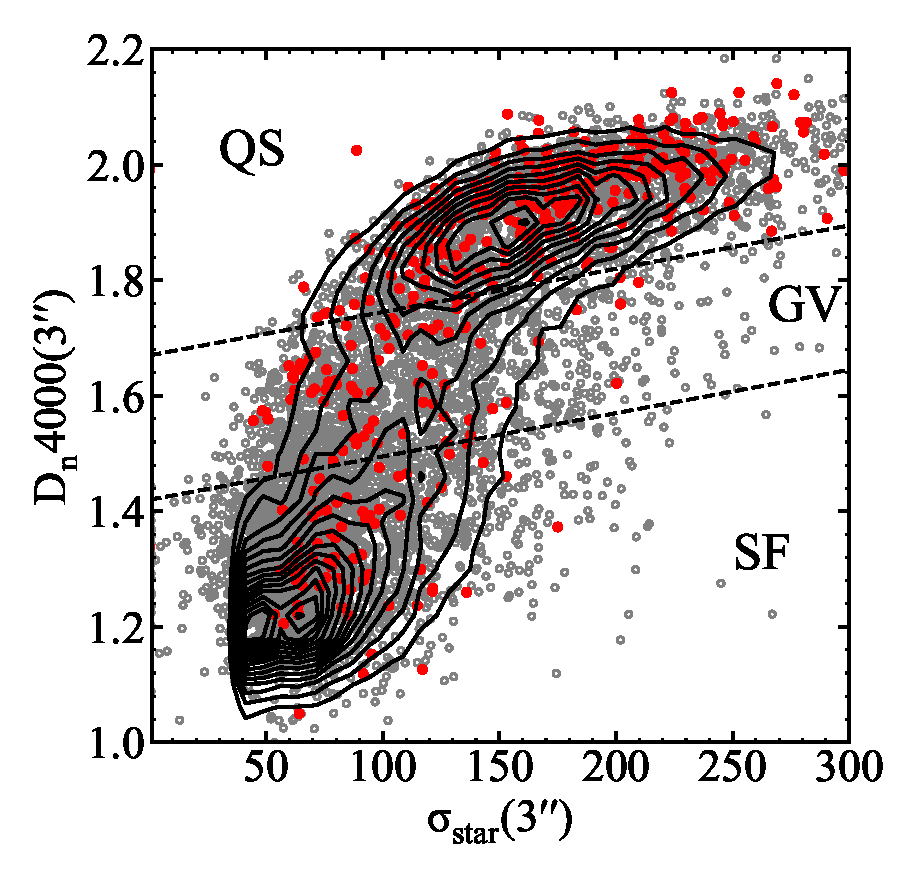
\includegraphics[width=\columnwidth]{pics/contour_Dn4000_V_DISP_3arcsec-3arcsec.eps}
    \caption{Diagram of central $3^{\prime \prime}$ D$_n$4000 versus ${\sigma}_{\rm star}$ for misaligned galaxies (red dots) and MaNGA sample (grey circles), with the SDSS DR7 sample shown as contours. There are two number density peaks in the contour. The two black dashed lines separate galaxies into star forming, green valley and quiescent sequence galaxies. The top dashed line is an approximation of the lower boundary of star forming main sequence (at the $\sim$1$\sigma$ level in scatter), while the bottom dashed line is an approximation of the upper boundary of quiescent sequence.}
    \label{fig:contour_Dn4000_V_DISP_3arcsec-3arcsec}
\end{figure}

\begin{table}
    \caption{Classification result of aligned/misaligned galaxies.}
    \label{tab:classification result}
    \begin{tabular}{lcc}
        \hline
        Aligned/Misaligned & Type & Number \\
        \hline
        Aligned & & 6502\\
        Misaligned & & \\
         & SF & 72\\
         & GV & 142\\
         & QS & 242\\
        Total & & 6958\\
        \hline
    \end{tabular}
\end{table}

\begin{figure}
    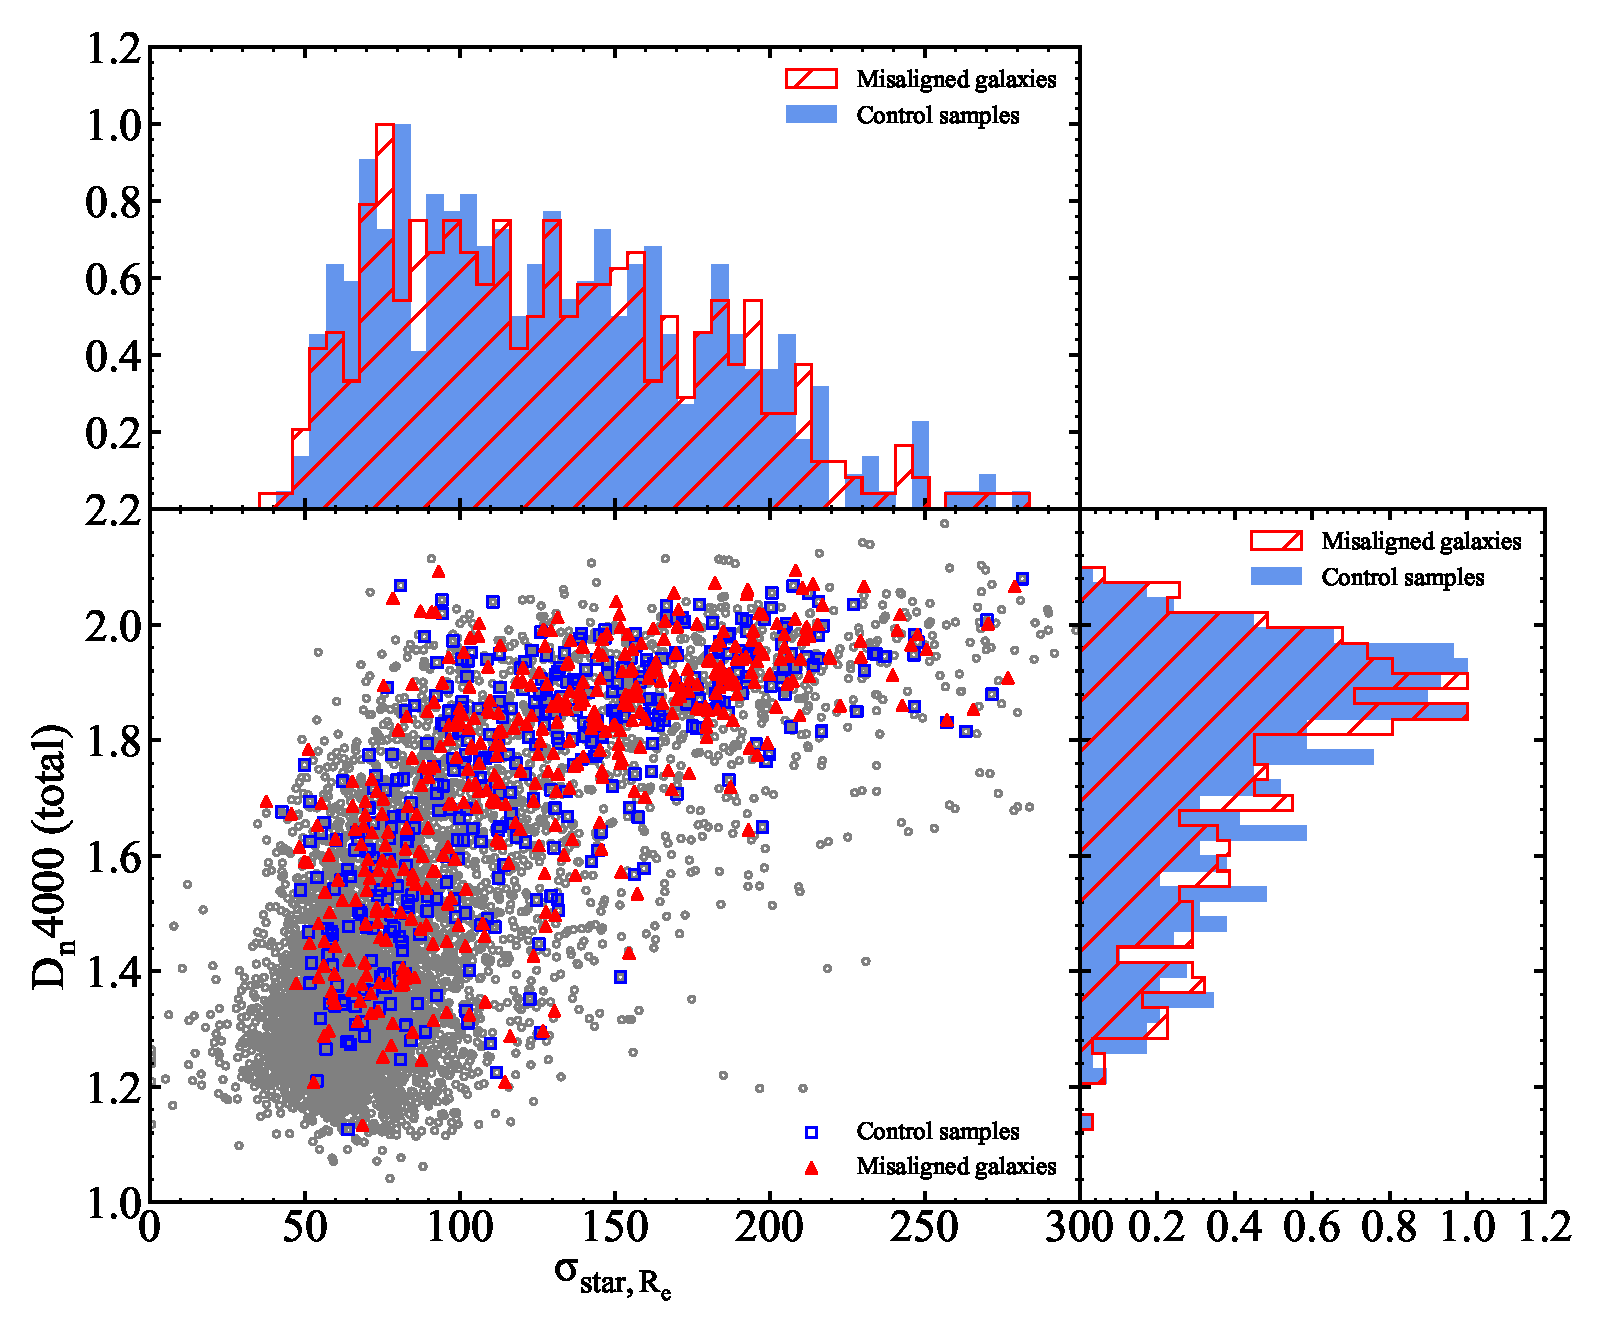
\includegraphics[width=1.0\columnwidth]{pics/Dn4000_sigma.eps}
    \caption{Total D$_n$4000 versus $\sigma_{{\rm star}, R_{\rm e}}$ for misaligned galaxies (red triangles) and one control sample (blue squares). The MaNGA galaxies are shown as grey circles. The top and right histograms show distribution of $\sigma_{{\rm star}, R_{\rm e}}$ and D$_n$4000, respectively. In each panel, the histograms filled with red lines are for the kinematically misaligned galaxies and that filled with blue color are for the control sample. The peaks of the distributions are set to 1.0.}
    \label{fig:Dn4000_sigma_star}
\end{figure}

The MaNGA sample and data products used in this work are drawn from the internal MaNGA Product Launch-10 (MPL-10), which includes 9456 unique galaxies. The MaNGA data analysis pipeline \citep[DAP,][]{westfall2019data} uses pPXF \citep{cappellari2004parametric} and a subset of stellar templates  from MaSTar library \citep{yan_sdss-iv_2019} to fit the stellar continuum in each spaxel. The data products include estimation of the stellar absorption and measurements of 21 major nebular emission lines in 3600$-$10,300 \r{A}, emission line fluxes are corrected for underlying stellar continuum absorption. The parameters we extracted from MaNGA DAP products named as "SPX-GAU-MILESCH-MASTARHC2", including : line-of-sight rotation velocity of stars ($V_{\rm star}$), stellar velocity dispersion (${\sigma}_{\rm star}$), line-of-sight rotation velocity of ionized gas ($V_{\rm gas}$), gas velocity dispersion (${\sigma}_{\rm gas}$), emission line fluxes (e.g. $\oiii\lambda$5007, $\ha$), lick indexes such as D$_n$4000, which is defined as the flux ratio between two narrow bands of 3850$-$3950 and 4000$-$4000 \r{A}.

In order to quantify the kinematic misalignment between stellar and gas components, we require the galaxies to have robust measurements of emission lines. We first separate the MaNGA sample into emission line galaxies and "line-less" galaxies."line-less" galaxies are defined as galaxies with $\ha$ signal-to-noise ratio smaller than 3 for more than $90\%$ spaxels within $\sim$1.5 $R_{\rm e}$. For 6958 emission line galaxies, we fit the kinematic position angle (PA) to both stellar (${\rm PA}_{\rm star}$) and gas (${\rm PA}_{\rm gas}$) velocity fields. The kinematic PA is measured based on established methods of \citet{krajnovic_kinemetry_2006}, it is defined as the counter-clockwise angle between north and a line that bisects the velocity field of gas or stars, measured on the receding side.

In Fig.~\ref{fig:explain_PA}, we show three examples of MaNGA galaxies. Each row represents a galaxy. The left panel shows the SDSS \textit{g,r,i}-band image (MaNGA ID is shown on the top), the middle panel shows the stellar velocity field and the right panel shows the velocity field of ionized gas traced by $\ha$. The values of rotation velocities are indicated by the color bar, the red side is moving away from us while the blue side is approaching us. The solid black and green lines in each velocity field show the kinematic major and minor axis fitted by Python module FIT\_KINEMATIC\_PA \citep{krajnovic_kinemetry_2006}, while two dashed lines show $\pm1\sigma$ error range. The top row shows a galaxy that has kinematically aligned gas and stellar components with $\Delta$PA = $1^{\circ}$; the middle row shows a galaxy with gas and stars rotating perpendicularly with $\Delta$PA $= 76^{\circ}$; the bottom row shows a counter-rotating galaxy with $\Delta$PA $= 167^{\circ}$. We identify 723 galaxies with robust PA measurement (error of PA < $60^{\circ}$) and $\Delta$PA $\ge 30^{\circ}$ as our kinematic decoupled sample. We eyeball both the photometry and velocity fields of these galaxies, removing irregular galaxies, broad line AGNs and on-going mergers. Finally the sample size is reduced to 456 galaxies.

Fig.~\ref{fig:contour_Dn4000_V_DISP_3arcsec-3arcsec} shows D$_n$4000-${\sigma}_{\rm star}$ relation for the central $3^{\prime \prime}$ of misaligned galaxies (red dots) and MaNGA galaxy sample (grey circles), with the SDSS DR7 sample shown as contours. The value of D$_n$4000 and ${\sigma}_{\rm star}$ within $3^{\prime \prime}$ are taken from MPA/JHU catalogue\footnote{https://wwwmpa.mpa-garching.mpg.de/SDSS/DR7/}. There are two density peaks in the contour. The peak at the bottom-left with lower D$_n$4000 and $\sigma_{\rm star}$ corresponds to younger stellar population, we refer them as star-forming (SF), the peak at the top-right with higher D$_n$4000 and $\sigma_{\rm star}$ corresponds to older stellar population, we refer them as quiescent sequence (QS). The population in between SF and QS is referred as green-valley (GV). The two black dashed lines separate these three populations. The top dashed line is an approximation of the lower boundary of star forming main sequence (at the $\sim$1$\sigma$ level in scatter), while the bottom dashed line is an approximation of the upper boundary of quiescent sequence. The classification result is listed in Table.~\ref{tab:classification result}. The reason that we do not apply the widely used SFR-$M_*$ relation to separate SF, GV, QS populations, includes: (1) different from SFR, D$_n$4000 can be measured consistently for all galaxies \citep{chen_post-starburst_2019}; (2) we hope to avoid any potential influence on the measurement of emission line strength due to the interaction between pre-existing and accreted external gas; (3) we find the median stellar velocity dispersion of the misaligned samples is 20$\sim$30 km$\rm \, s^{-1}$ larger than a control sample with similar D$_n$4000 and stellar mass distribution, considering that $\sigma_{\rm star}$ is a direct observed property that reflects the depth of the potential well of a galaxy \citep{2000ApJ...539L...9F, gebhardt2000relationship}, we use $\sigma_{\rm star}$ instead of $M_*$ in this work.

\subsection{Control sample}

It is believed that the gas components in the kinematically misaligned galaxies primarily originate from external processes like mergers and gas accretion. In order to understand the influence of external gas acquisition on the evolution of galaxies, we build control sample of galaxies with $\Delta$PA $< 30^{\circ}$. For each misaligned galaxy, we find ten non-misaligned galaxies which are closely matched in $\sigma_{{\rm star}, R_{\rm e}}$ ($|\Delta{\sigma}_{{\rm star}, R_{\rm e}}| \leq 8$) and global D$_n$4000 ($|\Delta$D$_n$4000$| \leq 0.05$) to construct the control sample. $\sigma_{{\rm star}, R_{\rm e}}$ is the stellar velocity dispersion at $R_{\rm e}$. Global D$_n$4000 is measured from the global spectrum within MaNGA bundle.

Fig.~\ref{fig:Dn4000_sigma_star} shows the misaligned sample (red triangles) and the control sample (blue squares) on the total D$_n$4000 versus $\sigma_{{\rm star}, R_{\rm e}}$ plane. The top and right histograms show distribution on $\sigma_{{\rm star}, R_{\rm e}}$ and D$_n$4000, respectively. It is clear that misaligned galaxies and control sample have the same distribution on $\sigma_{{\rm star}, R_{\rm e}}$ and total D$_n$4000.

Through quantifying the difference between the misaligned galaxies and the control sample, our aim is to have an idea about how the external processes influence galaxies evolution. 
